\chapter{Implementation}

\section{Authentication Policy}
With regard to the design of the authentication policies, conditional flows are used to fulfill the requirements for authentication policies.
The main difference is the additional lifecycle management provided for them with particular validations.
Reusing existing components is beneficial in this case as the implementation is simplified without introducing any other similar components.

In order to differentiate authentication flow and authentication policy, the parent authentication flow \textit{Authentication policies - PARENT} is provided to contain only authentication policies.
Moreover, every policy has the prefix \textit{"POLICY - "} for its alias to mark it as the authentication policy.
The validation and management for authentication policies are done through the specific \textit{Data Access Object} (DAO), shown in Section \ref{impl-authn-policies-dao}. 

As the authentication policies need to be managed from the outside world, the \textit{REST API} has been introduced with a detailed description in Section \ref{impl-authn-policies-rest}.
The administrator console, as a client application, also uses the Keycloak REST API to manage all entities.
More details about the administrator console interface are in Section \ref{impl-authn-policies-admin}.

\begin{figure}[htbp]
  \centering
  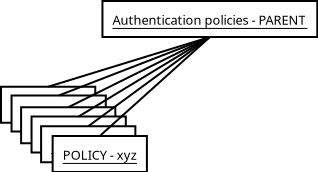
\includegraphics[width=0.5\textwidth]{img/sections/6-implementation/auth-policies-parent.png}
  \label{fig:impl-authn-policies-parent}
  \caption{Authentication Policies Parent}
\end{figure}

\newpage

\subsection{Data Access Object} \label{impl-authn-policies-dao}
A Data Access Object (DAO) pattern in software engineering abstracts database operations, shielding application logic from database sophistication and adhering to the single responsibility principle. //TODO Wikipedia

It is used to manage authentication policies as part of the separation from the authentication flows.
It provides necessary validation above the database layer and provides the functionality to properly mark conditional flow as an authentication policy.

The signature of operations for the authentication policy DAO is declared via the \textit{AuthnPolicyProvider} as shown in Figure \ref{fig:impl-authn-policies-provider-diagram}.

\begin{figure}[htbp]
  \centering
  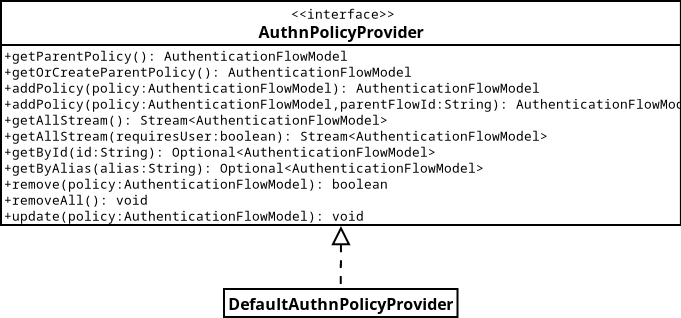
\includegraphics[width=1\textwidth]{img/sections/6-implementation/authn-policy-provider-diagram.png}
  \label{fig:impl-authn-policies-provider-diagram}
  \caption{Authentication Policy Provider}
\end{figure}

\newpage

The interface \textit{AuthnPolicyProvider} consists of the basic CRUD operations that can be made on authentication policies, such as:

\begin{itemize}
    \item \textit{getParentPolicy()} -- retrieve the parent \textit{Authentication policies - PARENT} flow.
    \item \textit{getOrCreateParentPolicy()} -- retrieve, or create if it does not exist, the parent \textit{Authentication policies - PARENT} flow.
    \item \textit{addPolicy(policy)} -- add a new policy \textit{policy} with the default parent flow.
    \item \textit{addPolicy(policy, parentFlowId)} -- add a new policy \textit{policy} with the parent flow \textit{parentFlowId}.
    \item \textit{getAllStream()} -- retrieve a stream of all authentication policies.
    \item \textit{getAllStream(requiresUser)} -- retrieve a stream of all authentication policies with the execution phase equal to \textit{requiresUser} attribute.
    \item \textit{getById(id)} -- retrieve an authentication policy found by provided ID via the \textit{id} attribute.
    \item \textit{getByAlias(alias)} -- retrieve an authentication policy found by provided alias via the \textit{alias} attribute.
    \item \textit{remove(policy)} -- remove a policy defined in the \textit{policy} attribute.
    \item \textit{removeAll()} -- remove all authentication policies.
    \item \textit{update(policy)} -- update an authentication policy provided via the \textit{policy} attribute.
\end{itemize}

\newpage
\subsubsection{Add Authentication Policy}
One of the most interesting examples of implementing methods of the \textit{AuthnPolicyProvider} interface is the \textit{addPolicy()} method shown in Figure \ref{fig:impl-authn-policies-add-policy-diagram}.
That method is responsible for creating a new authentication policy based on the parameters.

\begin{figure}[htbp]
  \centering
  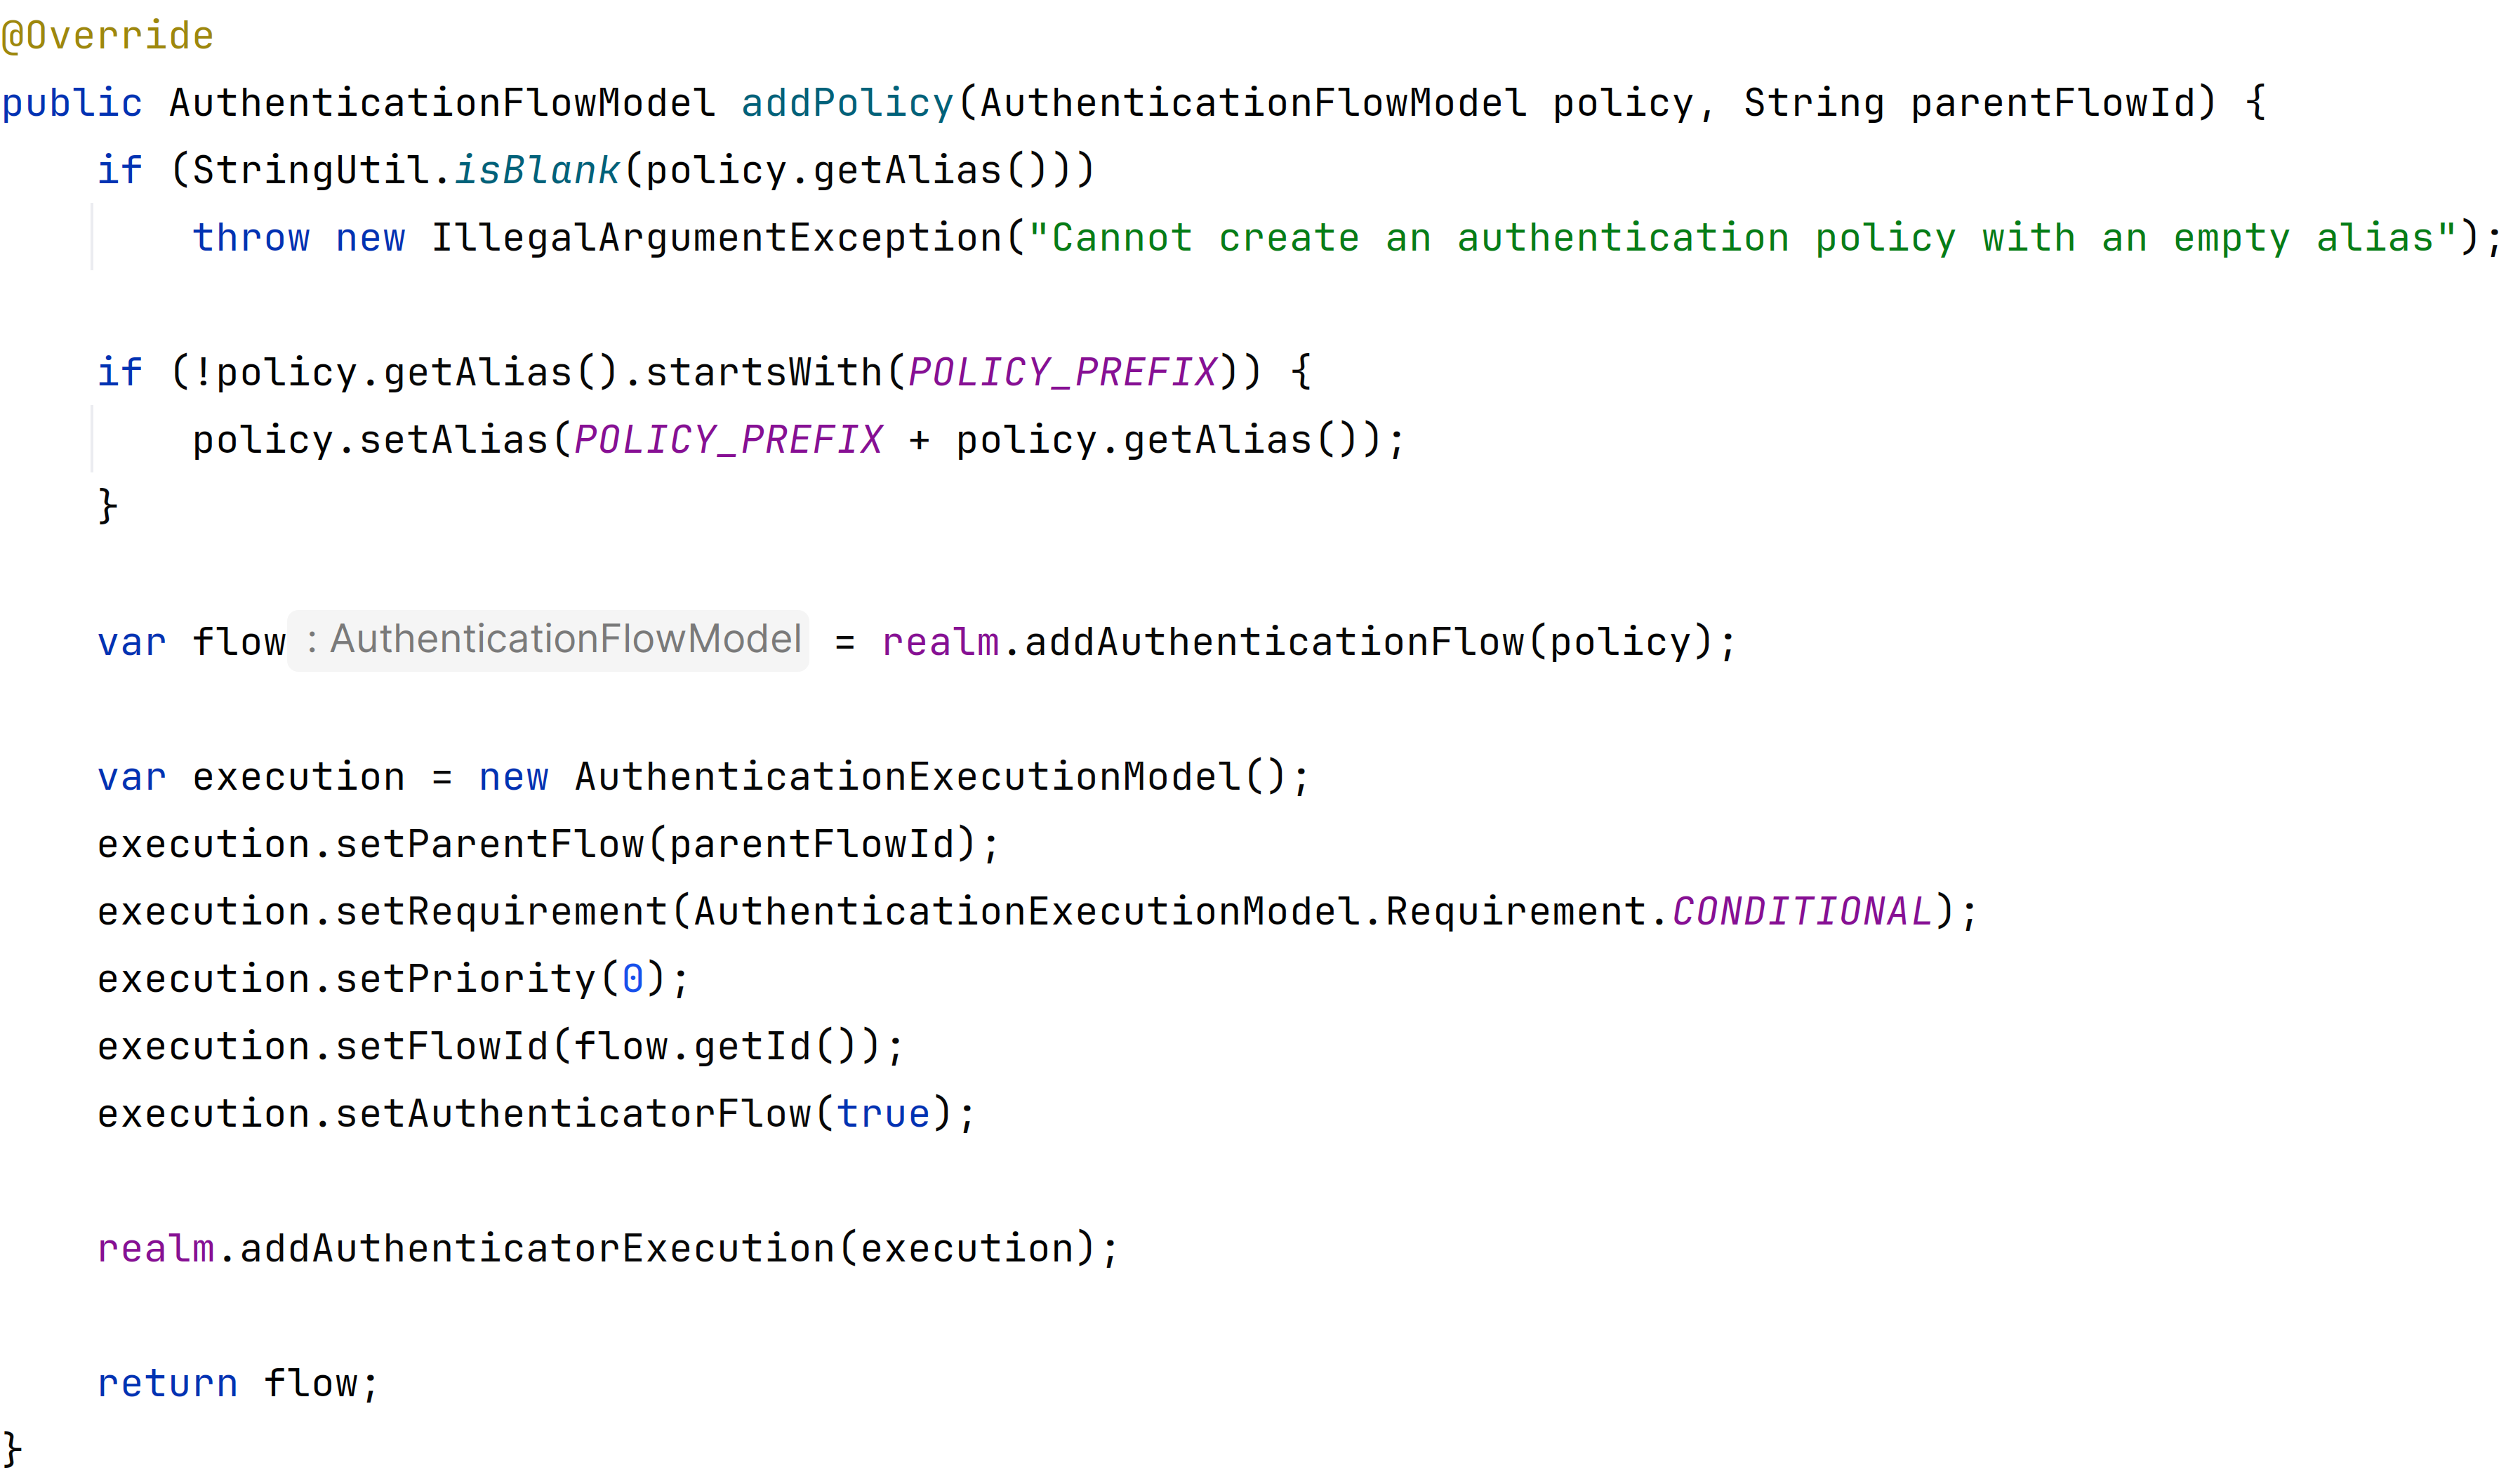
\includegraphics[width=1.05\textwidth]{img/sections/6-implementation/authnPolicyAddPolicy.png}
  \label{fig:impl-authn-policies-add-policy-diagram}
  \caption{Add Policy Method}
\end{figure}

First of all, the alias must not be empty.
Otherwise, the exception is thrown.
If the alias does not start with the prefix \textit{"POLICY - "}, it is automatically added to the alias.
The last part of the execution is to create a conditional flow where the parent flow is the common parent authentication flow for all authentication policies.
The newly created authentication policy is returned.

\newpage

\subsubsection{Retrieve Authentication Policies}

\begin{figure}[htbp]
  \centering
  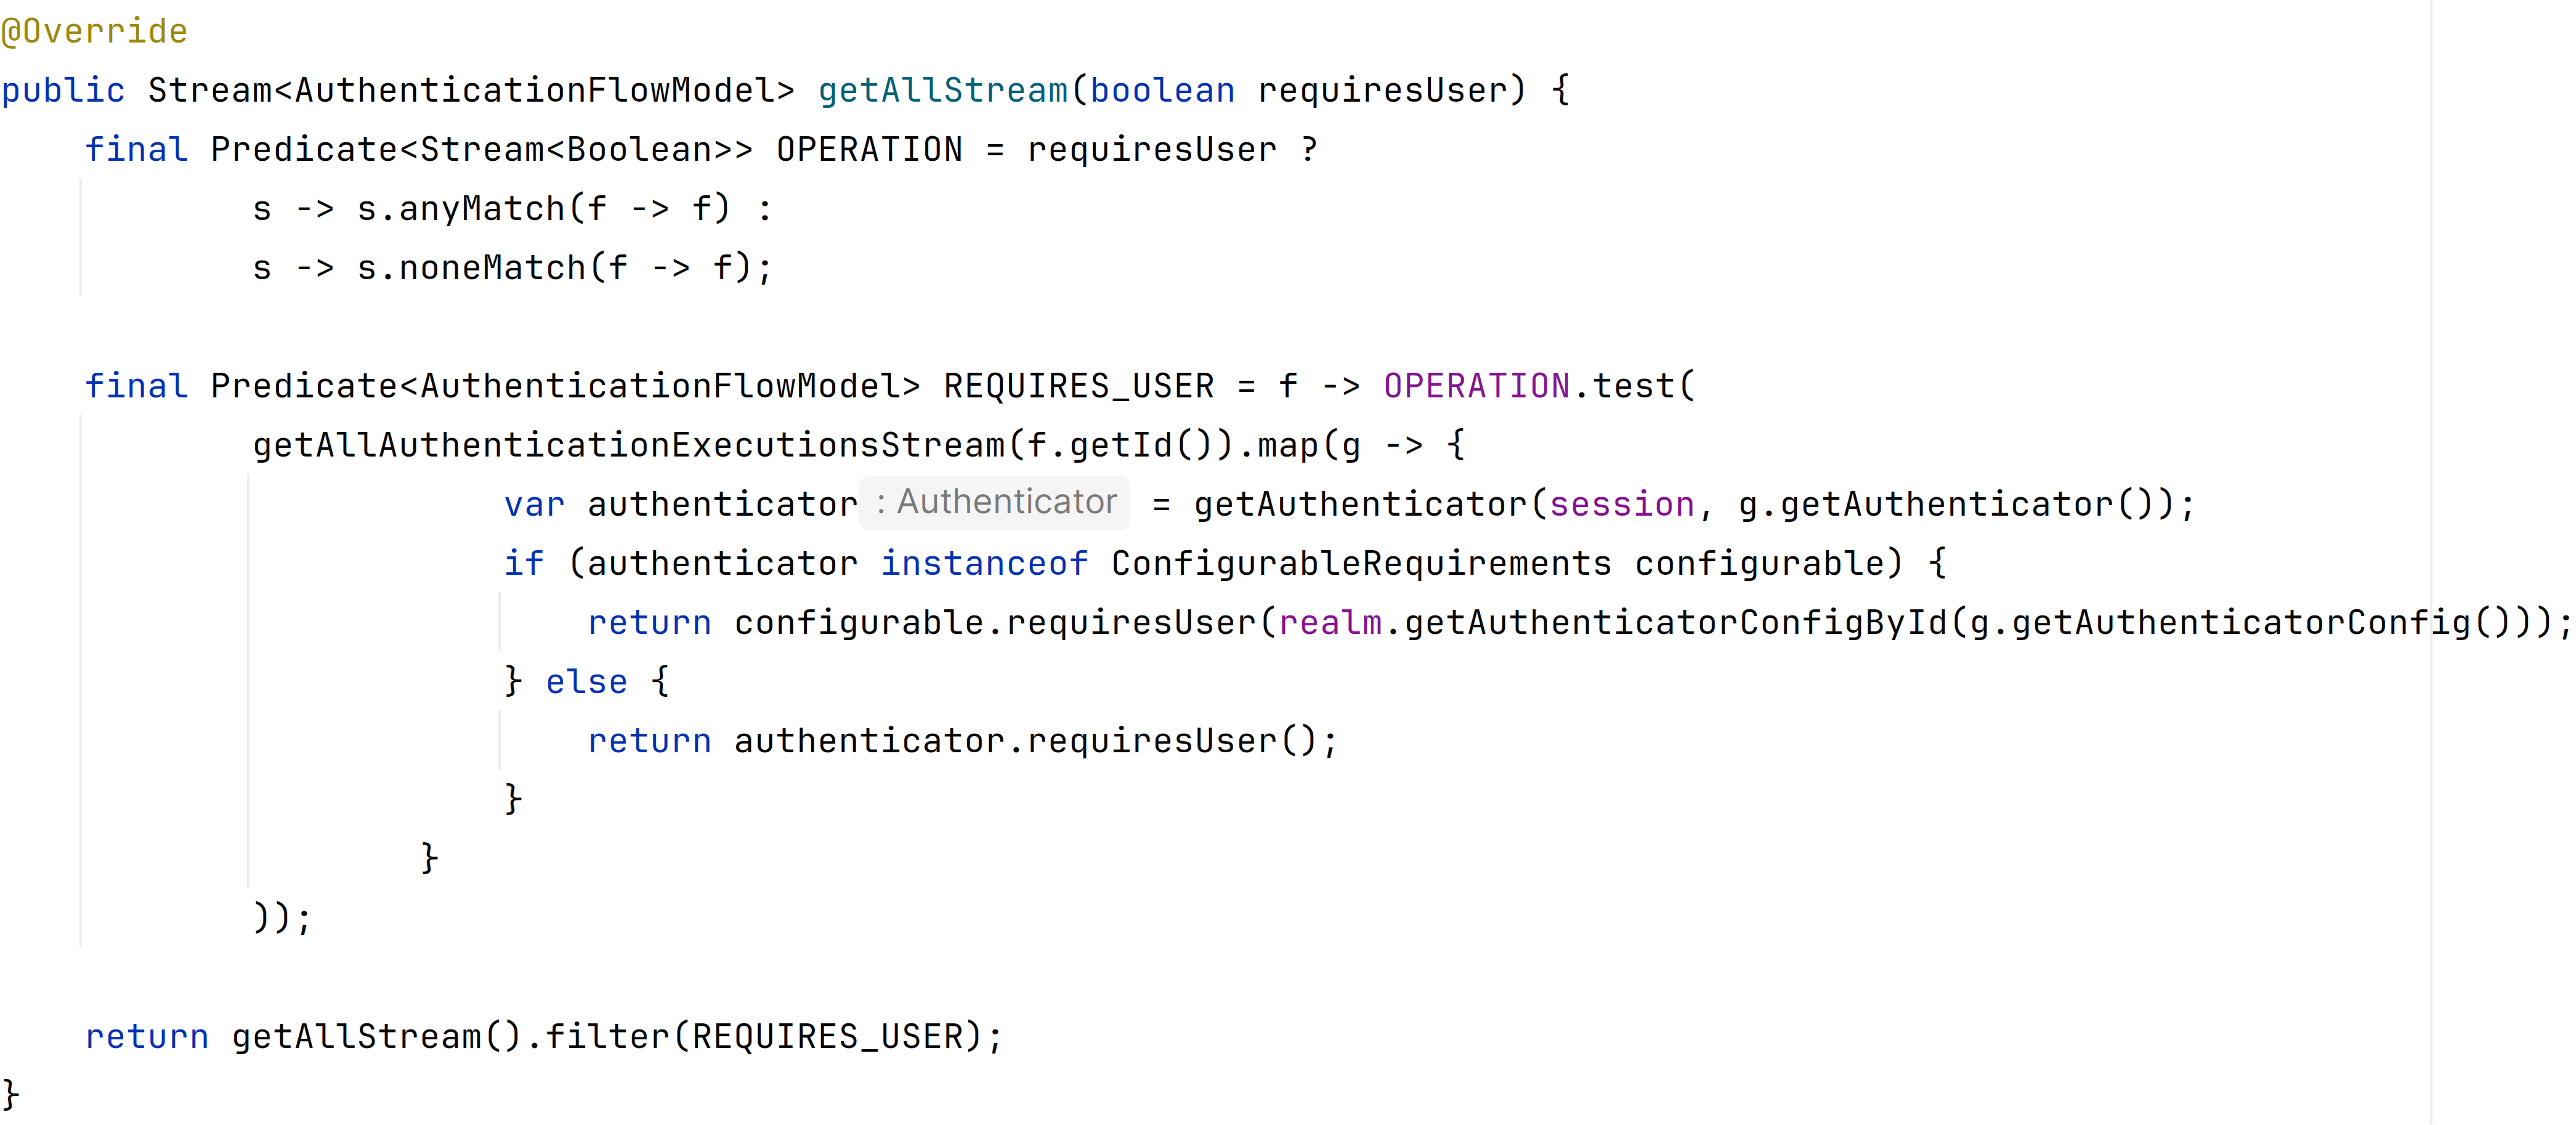
\includegraphics[width=1\textwidth]{img/sections/6-implementation/authnPolicyGetAllStream.png}
  \label{fig:impl-authn-policies-get-all}
  \caption{Get All Authentication Policies}
\end{figure}

\begin{figure}[htbp]
  \centering
  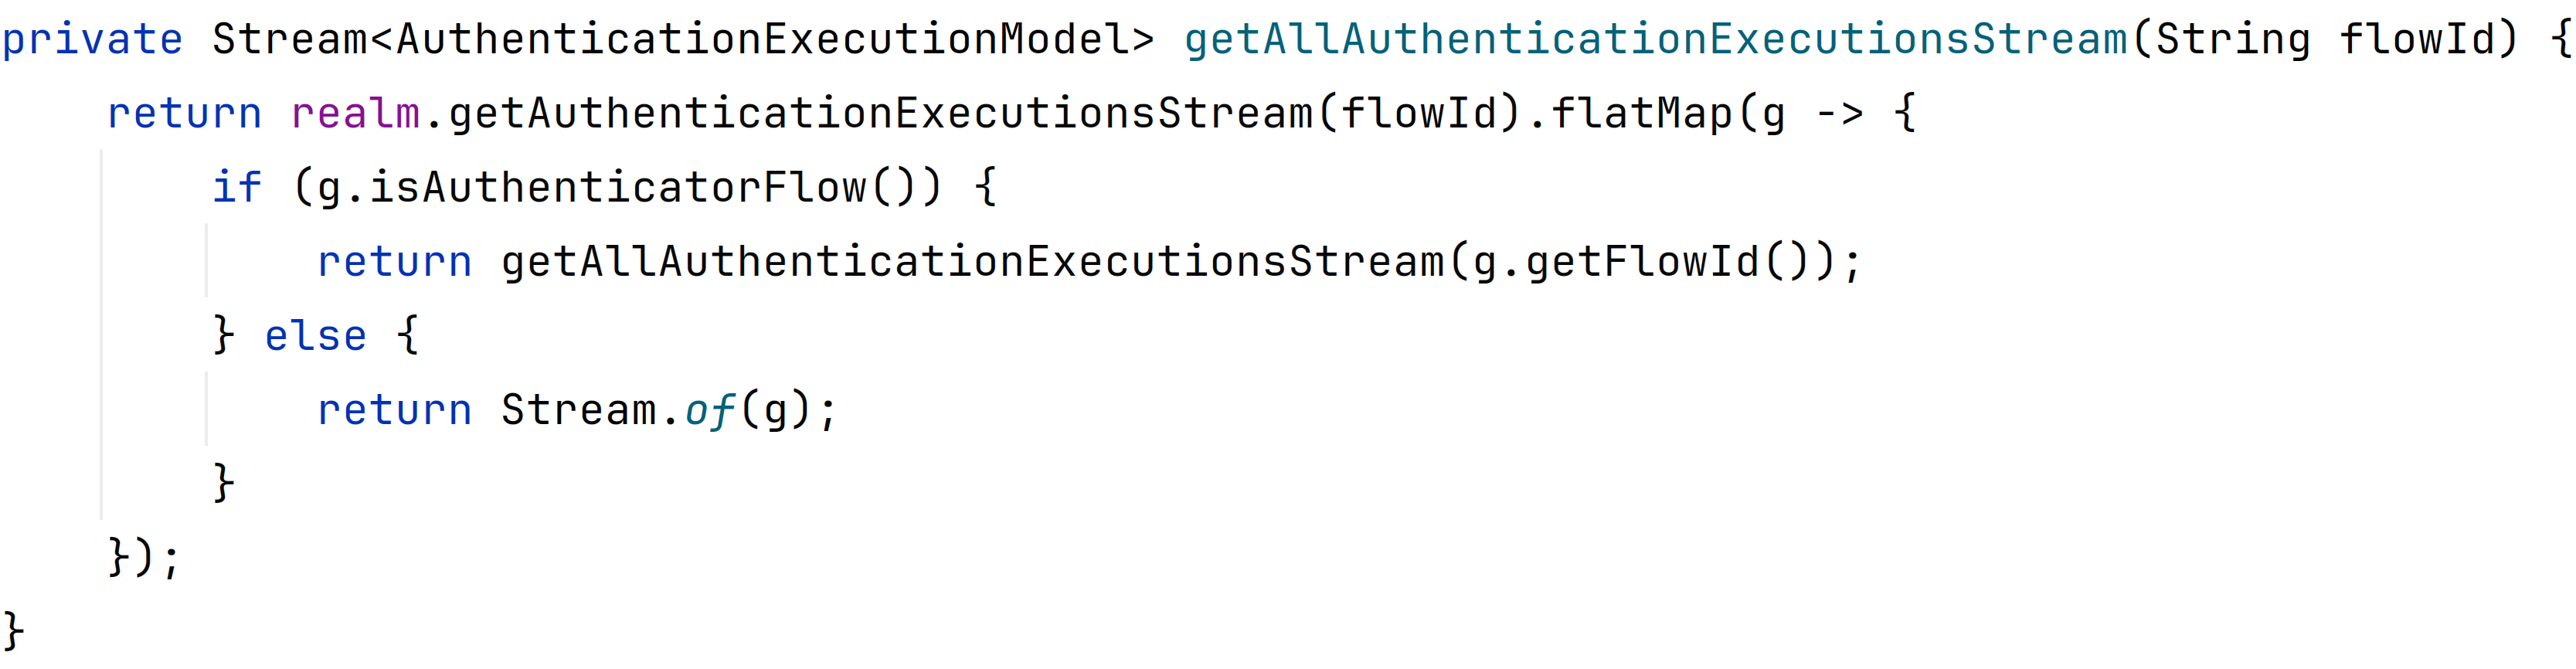
\includegraphics[width=1\textwidth]{img/sections/6-implementation/authnPolicyGetAllExecutions.png}
  \label{fig:impl-authn-policies-get-all-execs}
  \caption{Get All Authentication Executions}
\end{figure}


\newpage
\subsection{REST API} \label{impl-authn-policies-rest}
\subsection{Administrator Console} \label{impl-authn-policies-admin}

\section{User Context}

\section{User Context Condition}
\subsection{Operations Builder}

\section{User Evaluator}
\subsection{Configuration}

\section{User Engine}
\subsection{Asynchronous processing}
\subsection{Evaluation}
\subsection{Store Risk Score}

\section{Artificial Intelligence}

\section{External Integration}

\shorthandoff{-}